% =====================================================================
% Part I — TotD cluster A (permutation groups). Formalization pearl.
% Authors: Carles Marín (Claude, Anthropic, as AI assistant).
% Style: one message (a single counting identity unifies the cluster),
% story-driven, honest about scope, Lean names live in the tables.
% Clones the house line of godsil-gutman-lean.tex.
% Figures are TikZ; script-generated finals may replace them.
% =====================================================================
\documentclass[11pt]{article}
\usepackage[T1]{fontenc}
\usepackage{lmodern}
\usepackage{amsmath,amssymb,amsthm,booktabs,graphicx,hyperref}
\usepackage{xurl}
\usepackage[table]{xcolor}
\usepackage{pifont}
\usepackage{multirow}
\usepackage{tikz}
\usetikzlibrary{arrows.meta,positioning,calc,shapes.geometric}
\definecolor{sepblue}{HTML}{1B4F8C}
\definecolor{sepband}{HTML}{DCE3EB}
\definecolor{sepamber}{HTML}{E08A1E}
\definecolor{sepred}{HTML}{C0392B}
% categorical palette for the three canon voices (blue / amber / red-violet:
% distinguishable in greyscale and for common colour-vision deficiencies)
\definecolor{voiceA}{HTML}{1B6F8C}
\definecolor{voiceB}{HTML}{E08A1E}
\definecolor{voiceC}{HTML}{8C2D6F}
\definecolor{restgrey}{HTML}{B9C2CC}
% severity ramp for the distinguishing-number heatmap (D=2 calm -> D=4 alarm)
\definecolor{dTwo}{HTML}{DCE7EB}
\definecolor{dThree}{HTML}{F4C46B}
\definecolor{dFour}{HTML}{D9663A}
\usepackage[margin=1in]{geometry}
\usepackage{microtype}
\setlength{\emergencystretch}{2em}
\newtheorem{theorem}{Theorem}
\newtheorem{lemma}{Lemma}
\newtheorem{definition}{Definition}
\newcommand{\lean}[1]{\texttt{#1}}
\newcommand{\Z}{\mathbb{Z}}
\newcommand{\R}{\mathbb{R}}
\newcommand{\N}{\mathbb{N}}
\newcommand{\GL}{\mathrm{GL}}

\title{\bf When Separation Fails, a Canon Appears\\[3pt]
  \large\normalfont One counting identity behind separation, synchronization, and
  symmetry-breaking in permutation groups, formalized in Lean~4 (Part~I)}
\author{Carles Mar\'in\thanks{Formalized with AI assistance (Claude, Anthropic);
  the mathematics and all claims are the author's responsibility.}\\[3pt]
  \normalsize Independent researcher\\
  \normalsize \texttt{karlesmarin@gmail.com}}
\date{July 2026}

\begin{document}
\maketitle

\begin{abstract}
One arithmetic identity runs through this paper: the average, over a finite group
$G$ acting on $\Omega$, of how many points a translate $gA$ shares with a set $B$
is exactly $|A|\,|B|/|\Omega|$. Read one way it proves P.~M. Neumann's separation
lemma; read another it forces the uniformity theorems of P.~J. Cameron's
synchronization hierarchy; and at the boundary $|A|\,|B|=|\Omega|$ it yields a
dichotomy---either some $g$ pulls $A$ off $B$, or \emph{every} translate meets $B$
in exactly one point. That extremal case is an exact factorization of the group,
and over $\Z/n$ a rhythmic tiling canon: the boundary of separation theory and the
theory of musical canons are the same object, in two literatures that do not cite
one another. I formalize this cluster in Lean~4 / Mathlib, together with the
\emph{distinguishing number} of a group action and the Fano-plane value
$D(\GL_3(\mathbb{F}_2))=4$. The mathematics is classical; new here are the
orbit-local form of the dichotomy, the identification of its extremal case with
rhythmic canons, and---to my knowledge---the first formalization of any of these
in a proof assistant. Everything is \lean{sorry}-free, depending only on the three
standard axioms: a pearl, and the first part of a planned series.
\end{abstract}

% ---------------------------------------------------------------
\section{One argument, several faces}
\label{sec:intro}

Let a finite group $G$ act on a set $\Omega$, and take two finite subsets
$A,B\subseteq\Omega$. Applying $g\in G$ slides $A$ to its translate $gA$. Almost
everything in this paper follows from counting, in two ways, the triples
$(a,b,g)$ with $a\in A$, $b\in B$, and $g\cdot a=b$. When $G$ acts transitively on
$\Omega$, summing over the group and clearing denominators gives the identity
\[
  \boxed{\;\Bigl(\sum_{g\in G}|gA\cap B|\Bigr)\cdot|\Omega|
  \;=\;|A|\cdot|B|\cdot|G|\;}
\]
---the average size of $gA\cap B$ is $|A|\,|B|/|\Omega|$; a form local to the
orbits holds for any action, and is what the dichotomy of
Section~\ref{sec:dichotomy} needs. It looks like a
bookkeeping remark. It is in fact the engine of a surprisingly wide cluster of
theorems, and the single message of this paper is that they are one argument seen
from different sides (Figure~\ref{fig:map}).

\begin{figure}[t]
  \centering
  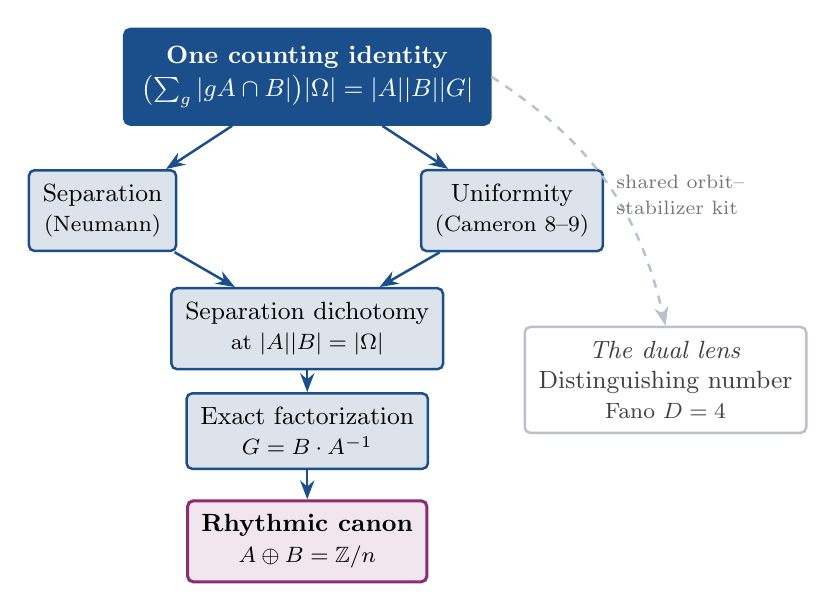
\begin{tikzpicture}[
      font=\small,
      box/.style={rounded corners=2pt,draw=sepblue,line width=0.9pt,fill=sepband,
                  align=center,inner sep=5pt,minimum height=8mm},
      hero/.style={rounded corners=2pt,draw=sepblue,line width=1.3pt,fill=sepblue,
                   text=white,align=center,inner sep=6pt},
      star/.style={rounded corners=2pt,draw=voiceC,line width=1.1pt,fill=voiceC!12,
                   align=center,inner sep=5pt},
      dual/.style={rounded corners=2pt,draw=restgrey,line width=0.9pt,fill=white,
                   align=center,inner sep=5pt,text=black!75},
      fl/.style={-{Stealth[length=2.4mm]},sepblue,line width=0.9pt}]
    \node[hero] (id) at (0,5.2) {\textbf{One counting identity}\\[1pt]
      $\bigl(\sum_g|gA\cap B|\bigr)|\Omega|=|A||B||G|$};
    \node[box] (sep) at (-2.6,3.5) {Separation\\{\footnotesize (Neumann)}};
    \node[box] (uni) at (2.6,3.5) {Uniformity\\{\footnotesize (Cameron 8--9)}};
    \node[box] (dic) at (0,2.0) {Separation dichotomy\\{\footnotesize at $|A||B|=|\Omega|$}};
    \node[box] (fac) at (0,0.7) {Exact factorization\\{\footnotesize $G=B\cdot A^{-1}$}};
    \node[star] (can) at (0,-0.7) {\textbf{Rhythmic canon}\\{\footnotesize $A\oplus B=\Z/n$}};
    \node[dual] (dist) at (4.55,1.35) {\emph{The dual lens}\\ Distinguishing number\\{\footnotesize Fano $D=4$}};
    \draw[fl] (id) -- (sep); \draw[fl] (id) -- (uni);
    \draw[fl] (sep) -- (dic); \draw[fl] (uni) -- (dic);
    \draw[fl] (dic) -- (fac); \draw[fl] (fac) -- (can);
    \draw[-{Stealth[length=2.4mm]},restgrey,line width=0.9pt,dashed]
      (id.east) to[bend left=22] node[right,midway,text=black!55,font=\scriptsize]{shared orbit--}
      node[right,midway,yshift=-3.2mm,text=black!55,font=\scriptsize]{stabilizer kit} (dist.north);
  \end{tikzpicture}
  \caption{The paper in one picture. A single counting identity forces both
  Neumann separation and Cameron's uniformity theorems; where they meet, at the
  threshold $|A||B|=|\Omega|$, it produces a dichotomy whose non-separable case is
  an exact factorization of the group---over $\Z/n$, a rhythmic tiling canon. The
  distinguishing number (the Fano exception $D=4$) is a parallel question about
  breaking symmetry, sharing the same orbit--stabilizer toolkit.}
  \label{fig:map}
\end{figure}

\paragraph{What is new, in three registers.} Because this paper sits between a
survey and a formalization, I separate its claims cleanly. \emph{Mathematically},
the new content is a sharpened, orbit-local form of the separation dichotomy
(Section~\ref{sec:dichotomy}), and the observation that its extremal case, over a
cyclic group, is exactly the rhythmic tiling canon of Vuza~\cite{Vuza1991} and
Coven--Meyerowitz~\cite{CovenMeyerowitz1999}.
\emph{In a proof assistant}: to the best of my knowledge, after an extensive
literature search across the major systems, this is the first formalization of the
separation lemma, of Cameron's synchronization hierarchy, and of the
distinguishing number of a group action. \emph{Conceptually}, the contribution is to make the shared engine
explicit: separation, uniformity, the extremal dichotomy, and the factorization
all reduce, by name and in the dependency graph, to the one identity above.
Appendix~\ref{app:results} lists the formal results with their Lean names; the
mathematics is classical throughout, and I name its authors as I go.

% Body table (Table 2: computational cross-checks) + shared status macros.
% Table 1 (formal results, Lean-heavy) lives in the appendix of the main file.
% Requires booktabs, amsmath/amssymb, xcolor[table]; colors sepblue/sepband,
% dTwo/dThree/dFour (defined in the main preamble).
\newcommand{\stproven}{\textcolor{sepblue}{\ding{51}}\,proven}
\newcommand{\stfuture}{\textcolor{restgrey}{$\circ$}\,future}
\newcommand{\stdef}{\textcolor{sepblue}{$\bullet$}\,defined}

% ---------- Table 2: computational cross-checks ----------
\begin{table}[t]
  \centering
  \small
  \arrayrulecolor{sepblue}
  \caption{Computational cross-checks (GAP / Sage, exact). \emph{Left:} the
  separation dichotomy, verified with no counterexample across every transitive
  group of small degree, plus the $\Z/12$ canon witness. \emph{Right:} an
  independent recomputation of Chan's distinguishing table
  $D(\GL_n(\mathbb{F}_q)\curvearrowright\mathbb{F}_q^n)$ for $n>2$, $q\le n{+}1$,
  matching Klavžar--Wong--Zhu; cell colour encodes $D$ (pale $D{=}2$ $\to$ deep
  $D{=}4$), so the two exceptions stand out at a glance.}
  \label{tab:checks}
  \renewcommand{\arraystretch}{1.2}
  \begin{minipage}[t]{0.46\textwidth}
    \centering
    \begin{tabular}{@{}ll@{}}
      \toprule
      \rowcolor{sepblue}
      \textcolor{white}{\textbf{Check}} & \textcolor{white}{\textbf{Result}} \\
      \midrule
      \rowcolor{sepband}
      dichotomy sweep & \multirow{1}{*}{0 counterexamples} \\
      \small 120 transitive grps, deg.\ 2--9 & \\
      $\Z/12$ canon $\{0,3,6,9\}{\oplus}\{0,1,2\}$ & tiles (extremal) \\
      \bottomrule
    \end{tabular}
  \end{minipage}\hfill
  \begin{minipage}[t]{0.5\textwidth}
    \centering
    \setlength{\tabcolsep}{5pt}
    \begin{tabular}{@{}c|cccc@{}}
      \multicolumn{1}{@{}c}{\scriptsize $n\backslash q$} & \scriptsize 2 & \scriptsize 3 & \scriptsize 4 & \scriptsize 5 \\
      \hline
      \scriptsize 3 & \cellcolor{dFour}\textbf{4} & \cellcolor{dTwo}2 & \cellcolor{dTwo}2 & --- \\
      \scriptsize 4 & \cellcolor{dThree}\textbf{3} & \cellcolor{dTwo}2 & \cellcolor{dTwo}2 & \cellcolor{dTwo}2 \\
      \scriptsize 5 & \cellcolor{dTwo}2 & \cellcolor{dTwo}2 & \cellcolor{dTwo}2 & \cellcolor{dTwo}2 \\
      \scriptsize 6 & \cellcolor{dTwo}2 & \cellcolor{dTwo}2 & \cellcolor{dTwo}2 & \cellcolor{dTwo}2 \\
    \end{tabular}
    \\[3pt]
    {\scriptsize\colorbox{dTwo}{\,$D{=}2$\,}\ \colorbox{dThree}{\,$D{=}3$\,}\ \colorbox{dFour}{\textcolor{white}{\,$D{=}4$\,}}\quad(``---'': $q$ not a prime power)}
  \end{minipage}
\end{table}


% ---------------------------------------------------------------
\section{Separating a set from its image}
\label{sec:setting}

The oldest face of the identity is a question with an intuitive answer:
\begin{quote}\itshape
  when can we always find a $g$ that pulls $A$ entirely off $B$---with
  $gA\cap B=\emptyset$?
\end{quote}
If the orbits are large there is room to slide $A$ clear of $B$. Neumann made
this precise. In the finite transitive case the clean threshold is
$|A|\cdot|B|<|\Omega|$: below it, separation is always possible
(Figure~\ref{fig:sep}); the counting identity is the whole proof, since if no $g$
separated then every term $|gA\cap B|\ge1$, forcing the sum to at least $|G|$ and
the average to at least $1$, i.e.\ $|A|\,|B|\ge|\Omega|$.

\begin{figure}[t]
  \centering
  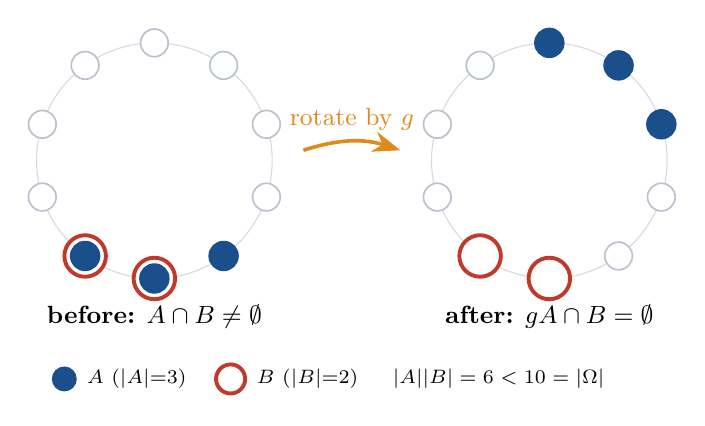
\begin{tikzpicture}[scale=0.88,
      pt/.style={circle,draw=restgrey,line width=0.6pt,fill=white,minimum size=10pt,inner sep=0pt},
      inA/.style={circle,draw=sepblue,line width=1pt,fill=sepblue,minimum size=10pt,inner sep=0pt},
      inB/.style={circle,draw=sepred,line width=1.4pt,fill=white,minimum size=15pt,inner sep=0pt}]
    \begin{scope}[shift={(0,0)}]
      \foreach \i in {0,...,9} { \coordinate (l\i) at ({90-36*\i}:1.7); }
      \draw[restgrey!60] (0,0) circle (1.7);
      \foreach \i in {0,...,9} { \node[pt] at (l\i) {}; }
      \foreach \i in {5,6} { \node[inB] at (l\i) {}; }
      \foreach \i in {4,5,6} { \node[inA] at (l\i) {}; }
      \node at (0,-2.25) {\small \textbf{before:} $A\cap B\neq\emptyset$};
    \end{scope}
    \draw[-{Stealth[length=3.5mm]},sepamber,line width=1.3pt]
      (2.15,0.15) to[bend left=18] node[above,midway,text=sepamber]{\small rotate by $g$} (3.55,0.15);
    \begin{scope}[shift={(5.7,0)}]
      \foreach \i in {0,...,9} { \coordinate (r\i) at ({90-36*\i}:1.7); }
      \draw[restgrey!60] (0,0) circle (1.7);
      \foreach \i in {0,...,9} { \node[pt] at (r\i) {}; }
      \foreach \i in {5,6} { \node[inB] at (r\i) {}; }
      \foreach \i in {0,1,2} { \node[inA] at (r\i) {}; }
      \node at (0,-2.25) {\small \textbf{after:} $gA\cap B=\emptyset$};
    \end{scope}
    \begin{scope}[shift={(-1.3,-3.15)}]
      \node[inA,scale=0.8] at (0,0) {}; \node[right=1pt,anchor=west] at (0.15,0) {\scriptsize $A$ ($|A|{=}3$)};
      \node[inB,scale=0.7] at (2.4,0) {}; \node[right=1pt,anchor=west] at (2.6,0) {\scriptsize $B$ ($|B|{=}2$)};
      \node[anchor=west] at (4.6,0) {\scriptsize $|A||B|=6<10=|\Omega|$};
    \end{scope}
  \end{tikzpicture}
  \caption{Separation on a decagon (regular $\Z/10$ action). Since
  $|A|\cdot|B|<|\Omega|$, some rotation slides $A$ (blue) off $B$ (red rings). The
  threshold $|A||B|=|\Omega|$, where separation can fail, is where the story turns
  (Section~\ref{sec:dichotomy}).}
  \label{fig:sep}
\end{figure}

One subtlety earns a sentence, because a popular paraphrase gets it wrong. The
threshold is \emph{strict}. The quantitative source---Birch, Burns, Oates
Macdonald and Neumann~\cite{BBMN1976}---separates under the hypothesis that every
orbit has \emph{more than} $|A|\,|B|$ elements, and notes that $|A|\,|B|+1$ is
best possible: a transitive group of degree $|A|\,|B|$ built from $|A|$ blocks of
size $|B|$ has a non-separable pair. Weakening ``more than'' to ``at least''
makes the statement false (the trivial group on one point never separates), and
the boundary case $|A|\,|B|=|\Omega|$---where the strict lemma is silent---is
exactly where Section~\ref{sec:dichotomy} lives.

For infinite $\Omega$ the right hypothesis is on orbits, and the sharp form asks
only that the orbit of every point of $A$ be infinite. The proof is the pleasant
dual of the finite one: if no $g$ separated, the cosets $\{g\mid g\cdot a=b\}$
would cover $G$, so by B.~H. Neumann's covering lemma~\cite{BHNeumann1954} some point stabilizer would
have finite index---but its index is the (infinite) orbit size. Mathlib already
carries B.~H. Neumann's covering lemma; the group-action wrapper it was missing is
supplied here.

% ---------------------------------------------------------------
\section{Uniformity: the same average, read as an equality}
\label{sec:engine}

Cameron's synchronization lectures~\cite{CameronSync} turn the identity into a family of rigidity
statements. If every translate-intersection happens to have the \emph{same} size
$\ell$, the identity immediately gives $|A|\,|B|=\ell\,|\Omega|$; its $\ell=1$
instance says a section-regular partition is uniform, every part the same size.
Sharper, and the fact that drives the next section: if all the intersections are
merely $\ge\ell$ (or all $\le\ell$) while $|A|\,|B|=\ell\,|\Omega|$, then every
one of them equals $\ell$ exactly.

The remarkable point is worth stating in plain words. An average is a statement
about a \emph{sum}; here it reaches down and pins every individual term. Because
the mean of the $|gA\cap B|$ is forced to be exactly $\ell$, no single translate
can sit above or below it without another compensating---so once a one-sided
bound removes that freedom, the average dictates each term on its own. It is an
average that legislates pointwise.

I am careful about what this ``unification'' is. I did not prove one meta-theorem
with separation, uniformity, and the dichotomy as corollaries; rather, all three
call the same triple-count. The unity is real but modest, and it lives in the
dependency graph, not in a grand statement---which is precisely the kind of claim
a formalization lets a reader check rather than take on faith.

% ---------------------------------------------------------------
\section{When separation fails: a dichotomy, and a canon}
\label{sec:dichotomy}

Return to the boundary $|A|\cdot|B|=|\Omega|$, where the strict separation lemma
says nothing. Here the engine forces a clean fork.

\begin{theorem}[Separation dichotomy, orbit-local form]
Let $G$ be finite acting on $\Omega$, and $A,B$ nonempty finite with every orbit
meeting both $A$ and $B$ of size $\ge|A|\cdot|B|$. Then either
\begin{enumerate}
\item[\rm(1)] some $g$ separates $A$ from $B$, or
\item[\rm(2)] \emph{(extremal)} $|gA\cap B|=1$ for \emph{every} $g\in G$, and $A$
  and $B$ lie in a single common orbit of size exactly $|A|\cdot|B|$.
\end{enumerate}
\end{theorem}

The proof is the average once more: if no $g$ separates, every term is $\ge1$; the
identity fixes their mean at $1$; so by the pointwise squeeze of the previous
section every $|gA\cap B|$ is exactly $1$, and the equality case collapses
$A\cup B$ into one orbit of the extremal size. Strictly above threshold one gets
separation outright.

I state the honesty plainly, because the fork's transitive core is not mine. That
$|A|\,|B|=|\Omega|$ forces either separation or all-intersections-one is,
essentially verbatim, the definition of a \emph{separating group} in
Araújo--Cameron--Steinberg~\cite{ACS2017}. What I claim is the orbit-local, weak,
non-transitive form above---the hypothesis constrains only the orbits meeting both
sets, and the conclusion \emph{produces} the single common orbit---and its
formalization.

\paragraph{The extremal case is a factorization.} What are the extremal pairs?
For the regular action of $G$ on itself, ``$|gA\cap B|=1$ for all $g$'' says
exactly that every group element is uniquely $b\,a^{-1}$ with $a\in A$, $b\in B$:
an \emph{exact factorization} $G=B\cdot A^{-1}$. Written additively for $G=\Z/n$ it
makes the difference map $(a,b)\mapsto b-a$ a bijection; equivalently, since
$|A|\,|B|=n$, the translates $\{A+b : b\in B\}$ partition $\Z/n$---the tiling
$A\oplus B=\Z/n$. Such a tiling is a \emph{rhythmic canon}: a rhythm $A$ and a set
of entry times $B$ whose shifted copies cover every beat once, with no gap and no
clash (Figure~\ref{fig:canon}). A non-separable extremal pair \emph{is} a canon.

\begin{figure}[t]
  \centering
  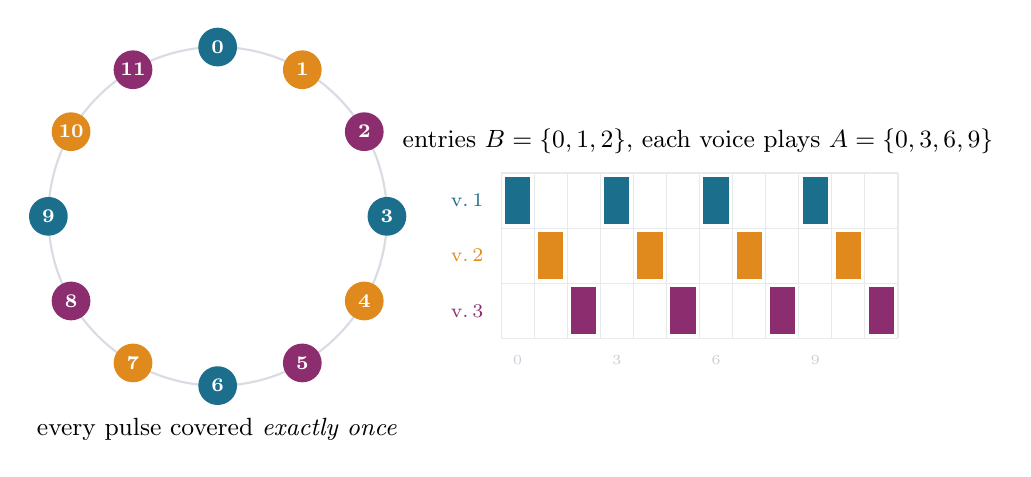
\begin{tikzpicture}[scale=1.0]
    \begin{scope}[shift={(-3.4,0)}]
      \draw[restgrey!55,line width=0.8pt] (0,0) circle (2.15);
      \foreach \i in {0,...,11} { \coordinate (c\i) at ({90-30*\i}:2.15); }
      \foreach \i in {0,3,6,9}  { \fill[voiceA] (c\i) circle (7pt); }
      \foreach \i in {1,4,7,10} { \fill[voiceB] (c\i) circle (7pt); }
      \foreach \i in {2,5,8,11} { \fill[voiceC] (c\i) circle (7pt); }
      \foreach \i in {0,...,11} { \node[white,font=\scriptsize\bfseries] at (c\i) {\i}; }
      \node at (0,-2.7) {\small every pulse covered \emph{exactly once}};
    \end{scope}
    \begin{scope}[shift={(0.2,-1.55)}]
      \foreach \t in {0,...,12} { \draw[restgrey!35,line width=0.4pt] (\t*0.42,0) -- (\t*0.42,2.1); }
      \foreach \r in {0,1,2,3} { \draw[restgrey!35,line width=0.4pt] (0,\r*0.7) -- (5.04,\r*0.7); }
      \foreach \t in {0,3,6,9} { \node[font=\tiny,text=restgrey!80] at (\t*0.42+0.21,-0.28) {\t}; }
      \foreach \t in {0,3,6,9}  { \fill[voiceA] (\t*0.42+0.05,1.45) rectangle (\t*0.42+0.37,2.05); }
      \foreach \t in {1,4,7,10} { \fill[voiceB] (\t*0.42+0.05,0.75) rectangle (\t*0.42+0.37,1.35); }
      \foreach \t in {2,5,8,11} { \fill[voiceC] (\t*0.42+0.05,0.05) rectangle (\t*0.42+0.37,0.65); }
      \node[left,font=\scriptsize,text=voiceA] at (-0.1,1.75) {v.\,1};
      \node[left,font=\scriptsize,text=voiceB] at (-0.1,1.05) {v.\,2};
      \node[left,font=\scriptsize,text=voiceC] at (-0.1,0.35) {v.\,3};
      \node[font=\scriptsize] at (2.5,2.5) {\small entries $B=\{0,1,2\}$, each voice plays $A=\{0,3,6,9\}$};
    \end{scope}
  \end{tikzpicture}
  \caption{The extremal (non-separable) pair $A=\{0,3,6,9\}$, $B=\{0,1,2\}$ on
  $\Z/12$ is a rhythmic canon. Left: the three translates $A$ (teal), $A{+}1$
  (amber), $A{+}2$ (violet) partition the twelve pulses---no gap, no overlap.
  Right: as music, three voices enter one beat apart, each playing the rhythm
  $A$. A sonified version accompanies the companion music-theory note.}
  \label{fig:canon}
\end{figure}

I flag the near neighbors so a referee need not. The idea ``non-separation $=$
factorization'' appears, for diagonal actions, in
Araújo--Cameron--Steinberg~\cite{ACS2017} (perfect factorizations of simple
groups), and for the $A=B$ case in Barbieri et~al.~\cite{Barbieri2025}
(difference sets and projective planes). What seems unremarked is the
identification of the two-set regular extremal case over $\Z/n$ with rhythmic
tiling canons: the separation literature and the tiling literature
(Vuza~\cite{Vuza1991}, Coven--Meyerowitz~\cite{CovenMeyerowitz1999},
Amiot~\cite{Amiot2016}) do not cite one another. The connection is novel as an
\emph{observation}, not as mathematics; its value is that it is now a lemma rather
than an analogy---which is what a proof assistant is for.

% ---------------------------------------------------------------
\section{The dual question: how much symmetry must you break?}
\label{sec:distinguishing}

So far the counting engine has measured how a group \emph{moves} sets---how far it
can push $A$ off $B$. A mirror quantity measures how hard the action is to
\emph{pin down}: how much labeling it takes to remove its symmetry entirely. I
view the two as opposite ends of one programme---separation adds room until the
group can move a set clear; distinguishing adds colours until the group can move
nothing at all---and a single inequality proved below joins them: a base of size $b$ (a set
whose pointwise stabilizer is trivial) gives $D\le b+1$, the bound that ties
distinguishing to the base and matroid theory (IBIS) forming the spine of Part~II.
That is why the topic belongs here, as the counting programme's dual face rather
than an appendix.

Color the points of $\Omega$; the coloring is \emph{distinguishing} if the
identity is the only element of $G$ that preserves it, and the \emph{distinguishing
number} $D(G\curvearrowright\Omega)$ is the fewest colors that suffice
(Albertson--Collins~\cite{AlbertsonCollins1996}; Tymoczko~\cite{Tymoczko2004} for
general actions). Mathlib had no notion of it; the definition, its monotonicity,
and the base bound $D\le b+1$ are supplied here.

\begin{quote}\itshape
  For $\GL_n(\mathbb{F}_q)$ acting on the nonzero vectors of $\mathbb{F}_q^n$,
  how many colors does it take?
\end{quote}
Melody Chan asked exactly this~\cite{Chan2006}; the answer is
Klavžar--Wong--Zhu~\cite{KWZ2006}: two colors always suffice, with four
exceptions, of which the unique maximum is $D(\GL_3(\mathbb{F}_2))=4$. That group,
of order $168$, is the collineation group of the Fano plane on its seven points,
and the exceptional value is the one I verify (Figure~\ref{fig:fano}).

The surprise is the size of the gap. For every larger linear action two colors
break all the symmetry; here, on just seven points, even \emph{three} colors
cannot---every one of the $3^7=2187$ three-colorings is preserved by some
collineation---while a specific four-coloring does. The lower bound is the
exhaustive half: twenty-one collineations suffice to fix every three-coloring
between them, checked by the kernel. The upper bound is pure geometry: three
points wear unique colors and are pinned, three lines through them pin three more,
and injectivity pins the last. The Fano plane is small enough to see and just
large enough to be rigid.

\begin{figure}[t]
  \centering
  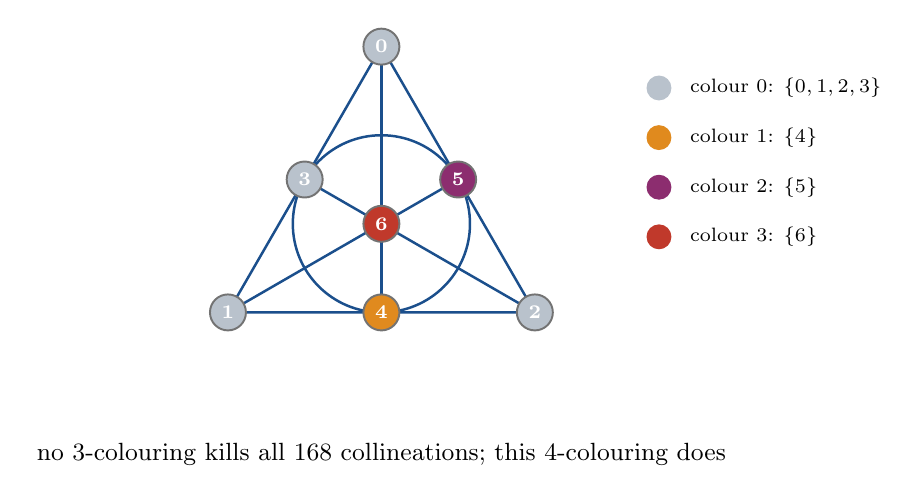
\begin{tikzpicture}[scale=1.5,
      fp/.style={circle,draw=black!55,line width=0.7pt,minimum size=13pt,inner sep=0pt,font=\scriptsize\bfseries}]
    \coordinate (P0) at (90:1.5);
    \coordinate (P1) at (210:1.5);
    \coordinate (P2) at (330:1.5);
    \coordinate (P3) at ($(P0)!0.5!(P1)$);
    \coordinate (P4) at ($(P1)!0.5!(P2)$);
    \coordinate (P5) at ($(P2)!0.5!(P0)$);
    \coordinate (P6) at (0,0);
    \draw[sepblue,line width=0.9pt] (P0)--(P1)--(P2)--cycle;
    \draw[sepblue,line width=0.9pt] (P0)--(P4); \draw[sepblue,line width=0.9pt] (P1)--(P5); \draw[sepblue,line width=0.9pt] (P2)--(P3);
    \draw[sepblue,line width=0.9pt] (P6) circle (0.75);
    \node[fp,fill=restgrey,text=white] at (P0) {0};
    \node[fp,fill=restgrey,text=white] at (P1) {1};
    \node[fp,fill=restgrey,text=white] at (P2) {2};
    \node[fp,fill=restgrey,text=white] at (P3) {3};
    \node[fp,fill=voiceB,text=white] at (P4) {4};
    \node[fp,fill=voiceC,text=white] at (P5) {5};
    \node[fp,fill=sepred,text=white]  at (P6) {6};
    \begin{scope}[shift={(2.35,1.15)},every node/.style={anchor=west,font=\scriptsize}]
      \fill[restgrey] (0,0) circle (3pt);   \node at (0.18,0) {colour 0: $\{0,1,2,3\}$};
      \fill[voiceB]  (0,-0.42) circle (3pt);\node at (0.18,-0.42) {colour 1: $\{4\}$};
      \fill[voiceC]  (0,-0.84) circle (3pt);\node at (0.18,-0.84) {colour 2: $\{5\}$};
      \fill[sepred]  (0,-1.26) circle (3pt);\node at (0.18,-1.26) {colour 3: $\{6\}$};
    \end{scope}
    \node[font=\small] at (0,-1.95) {no $3$-colouring kills all $168$ collineations; this $4$-colouring does};
  \end{tikzpicture}
  \caption{The Fano plane ($7$ points, $7$ lines), whose $168$ collineations are
  $\GL_3(\mathbb{F}_2)$ on the nonzero vectors of $\mathbb{F}_2^3$. The unique
  colours $1,2,3$ pin points $4,5,6$; three lines then pin $2,0,1$ and
  injectivity pins $3$. Hence $D=4$.}
  \label{fig:fano}
\end{figure}

% ---------------------------------------------------------------
\section{Why this matters}
\label{sec:why}

I address three readers directly, because the work speaks to each differently.

\paragraph{To a permutation-group theorist.} The extremal case of separation is
usually met as a curiosity at the boundary of a threshold theorem. Reading it as
an exact factorization, and then as a tiling, connects it to a large and active
body of work---Vuza's aperiodic canons~\cite{Vuza1991}, the Coven--Meyerowitz
conditions~\cite{CovenMeyerowitz1999}, Fuglede's spectral-set
question~\cite{Fuglede1974}---that the synchronization literature does not
currently draw on. The dictionary runs both ways: constructions of aperiodic
tilings become constructions of non-separable extremal pairs, and vice versa. The
orbit-local form of the dichotomy is also, I believe, the natural statement---it
needs neither transitivity nor a global orbit bound.

\paragraph{To someone building mathematics in Lean.} These foundations were not
previously available in a proof assistant. The averaging identity, the uniformity
theorems, the base bound $D\le b+1$, and the distinguishing-number API are now
reusable; they are exactly the pieces on which the matroid (IBIS) theory of
Part~II is built. Mathlib gains a small but load-bearing corner
of permutation-group combinatorics it did not have.

\paragraph{To someone in synchronization theory.} The separating/synchronizing
hierarchy is defined through precisely the intersection condition studied here.
Making the counting engine and the extremal dichotomy formal, and tying the
extremal case to a well-developed tiling theory, offers the field both a checked
foundation and a source of examples and non-examples it has not been mining. The
$\Z/n$ canons are an inexhaustible supply of extremal pairs.

% ---------------------------------------------------------------
\section{Where I stopped}
\label{sec:future}

This is the first cluster of a series, honestly mapped, not a finished theory.
Done: Neumann separation (finite and infinite); the counting engine and the
uniformity theorems; the orbit-local dichotomy with the factorization and
rhythmic-canon identification; distinguishing numbers, their API, and the Fano
exception. Ahead, and pinned but not yet built: the IBIS theorem of
Cameron--Fon-Der-Flaass~\cite{CFF1995} (irredundant bases of constant size are a matroid), the
central brick of Part~II and the natural home of the base bound proved here; the
explicit bridge lemmas that turn this cluster from a list into a fabric; and
Chan's remaining distinguishing values, together with the apparently untreated
projective analogue $D(\mathrm{PGL}_n(\mathbb{F}_q)\curvearrowright
\mathrm{PG}^{n-1})$. The road is classical, but unbuilt.

% ---------------------------------------------------------------
\section{Related work}
\label{sec:related}

The mathematics is classical: the separation lemma is Birch--Burns--Oates
Macdonald--Neumann~\cite{BBMN1976} and Neumann's infinite version; the counting
hierarchy and the separating/synchronizing dichotomy are Cameron's and
Araújo--Cameron--Steinberg's~\cite{ACS2017}; the $A=B$ extremal theory is
Barbieri et~al.~\cite{Barbieri2025}; distinguishing numbers are
Albertson--Collins and, for linear groups, Chan~\cite{Chan2006} and
Klavžar--Wong--Zhu~\cite{KWZ2006}; the tiling side is Vuza and Coven--Meyerowitz.
On the formal side, Mathlib provides group actions, orbit--stabilizer, Burnside,
matroids, and B.~H. Neumann's coset-covering lemma, but none of the separation
lemma, the synchronization hierarchy, or distinguishing numbers; I am aware of no
prior machine-checked treatment of these in any prover.

% ---------------------------------------------------------------
\section{Conclusion}

One counting identity, viewed through different lenses, generates separation,
synchronization, exact factorizations, rhythmic canons, and---through the dual
question of coloring---symmetry-breaking. Formalization does not create this
unity; it makes it explicit, and checkable, and it turns the crossing between
permutation groups and musical canons from an analogy into a theorem. None of the
mathematics is new; the contribution is that it now lives in a proof assistant,
and that the shared engine is visible in the dependency graph rather than
asserted. Each new piece arose from looking at the case a classical theorem leaves
aside---the equality in a strict inequality, the boundary of a threshold---which is
often where an unnamed object sits. I offer this as a pearl, and as the first part
of a series.

Part~II takes up the one brick this paper only names: the theorem of Cameron and
Fon-Der-Flaass that a permutation group whose irredundant bases all have the same
size carries a matroid on its points. It is the structural heart the base bound
$D\le b+1$ already points to, and with it the pieces gathered here---separation,
counting, uniformity, distinguishing---become a single connected chapter rather
than a first stone. The counting identity of Section~\ref{sec:intro} will still be
underneath; the aim of the series is to keep making such shared engines visible,
one checked brick at a time.

\paragraph{On method.} This development was carried out with AI assistance
(Claude, Anthropic): definitions, lemmas, and tactics were proposed and then
accepted or rejected against the kernel. The scope-keeping of this paper---the
classical cores named as such, the one value I could not feasibly prove in Lean
(the order $168$) flagged and cross-checked in GAP rather than asserted---reflects
that the kernel, not the assistant, has the last word.

\paragraph{Artifacts.} All Lean sources (\lean{sorry}-free; the axiom report is in
Table~\ref{tab:results}), the GAP cross-checks of Table~\ref{tab:checks}, and the
figures are available at
\url{https://github.com/karlesmarin/godsil-gutman-lean}, archived at
\textsc{doi}~\href{https://doi.org/10.5281/zenodo.21419285}{10.5281/zenodo.21419285}.

% ---------------------------------------------------------------
\appendix
\section{The formal results}
\label{app:results}

Table~\ref{tab:results} lists every formalized statement with its Lean name and
status. All theorems are \lean{sorry}-free and non-vacuous, and \lean{\#print
axioms} reports only \lean{propext}, \lean{Classical.choice}, \lean{Quot.sound}
(the exhaustive cover \lean{fanoWitnesses\_cover} needs even less). The three
\stfuture{} rows are the frontier mapped in Section~\ref{sec:future}.

\begin{table}[ht]
  \centering
  \small
  \arrayrulecolor{sepblue}
  \caption{The formalised results (Lean~4 / Mathlib).}
  \label{tab:results}
  \renewcommand{\arraystretch}{1.15}%

  \begin{tabular}{@{}lll@{}}
    \toprule
    \rowcolor{sepblue}
    \textcolor{white}{\textbf{Lean name}} & \textcolor{white}{\textbf{Statement}} & \textcolor{white}{\textbf{Status}} \\
    \midrule
    \rowcolor{sepband}
    \texttt{separation\_lemma\_of\_pretransitive} & $|A||B|<|\Omega|\Rightarrow\exists g,\ gA\cap B=\emptyset$ & \stproven \\
    \texttt{neumann\_separation\_lemma} & orbits of $A$ infinite $\Rightarrow$ separable & \stproven \\
    \rowcolor{sepband}
    \texttt{sum\_card\_smul\_inter\_mul\_card} & $(\sum_g|gA\cap B|)\,|\Omega|=|A||B||G|$ \; (Cameron Thm~10) & \stproven \\
    \texttt{card\_smul\_inter\_eq\_of\_forall\_le} & average-equals-extremum squeeze \; (Cameron Thm~8) & \stproven \\
    \rowcolor{sepband}
    \texttt{IsSectionRegular.card\_part\_mul\dots} & section-regular $\Rightarrow$ uniform \; (Cameron Thm~9) & \stproven \\
    \texttt{separation\_dichotomy} & separate, \emph{or} $|gA\cap B|{=}1\ \forall g$ on one $|A||B|$-orbit & \stproven \\
    \rowcolor{sepband}
    \texttt{\dots\_eq\_one\_iff\_factorization} & extremal $\iff$ exact factorization $G=B\cdot A^{-1}$ & \stproven \\
    \texttt{\dots\_vadd\_inter\_eq\_one\_iff\_tiling} & over $\Z/n$: extremal $\iff$ rhythmic tiling canon & \stproven \\
    \rowcolor{sepband}
    \texttt{distinguishingNumber} \small(+API) & least $k$ with a symmetry-killing $k$-colouring & \stdef \\
    \texttt{distinguishingNumber\_le\_card\_base\dots} & base of size $b\Rightarrow D\le b{+}1$ \; (bridge to IBIS) & \stproven \\
    \rowcolor{sepband}
    \texttt{fano\_distinguishingNumber} & $D(\GL_3(\mathbb{F}_2)\curvearrowright\mathbb{F}_2^3)=4$ & \stproven \\
    \midrule
    \emph{IBIS} (Cameron--Fon-Der-Flaass) & irredundant bases const.\ size $\iff$ matroid & \stfuture \\
    \emph{bridge lemmas} & separation $\leftarrow$ engine; extremal $=$ Thm~8 $\ell{=}1$ & \stfuture \\
    \emph{Chan full classification} & the $D{=}3$ cases; general $D{=}2$; $\mathrm{PGL}$ analogue & \stfuture \\
    \bottomrule
  \end{tabular}
  \arrayrulecolor{black}
\end{table}

\bibliographystyle{plain}
\begin{thebibliography}{99}
% --- separation / synchronization ---
\bibitem{BBMN1976} B.~J. Birch, R.~G. Burns, S. Oates Macdonald, P.~M. Neumann,
  \emph{On the orbit-sizes of permutation groups containing elements separating
  finite subsets}, Bull. Austral. Math. Soc. \textbf{14} (1976) 7--10.
\bibitem{BHNeumann1954} B.~H. Neumann, \emph{Groups covered by permutable
  subsets}, J. London Math. Soc. \textbf{29} (1954) 236--248.
\bibitem{ACS2017} J. Araújo, P.~J. Cameron, B. Steinberg, \emph{Between primitive
  and 2-transitive: synchronization and its friends}, EMS Surv. Math. Sci.
  \textbf{4} (2017) 101--184.
\bibitem{CameronSync} P.~J. Cameron, \emph{Synchronization}, lecture notes
  (LTCC), 2010; \url{https://cameroncounts.wordpress.com/lecture-notes/}.
\bibitem{Barbieri2025} M. Barbieri, P. Lekše, P. Potočnik, K. Rekvényi,
  \emph{Separating subsets from their images} (2025), arXiv:2508.20731.
% --- bases / matroids / distinguishing ---
\bibitem{CFF1995} P.~J. Cameron, D.~G. Fon-Der-Flaass, \emph{Bases for
  permutation groups and matroids}, European J. Combin. \textbf{16} (1995)
  537--544.
\bibitem{AlbertsonCollins1996} M.~O. Albertson, K.~L. Collins, \emph{Symmetry
  breaking in graphs}, Electron. J. Combin. \textbf{3} (1996) \#R18.
\bibitem{Tymoczko2004} J. Tymoczko, \emph{Distinguishing numbers for graphs and
  groups}, Electron. J. Combin. \textbf{11} (2004) \#R63.
\bibitem{Chan2006} M. Chan, \emph{The maximum distinguishing number of a group},
  Electron. J. Combin. \textbf{13} (2006) \#R70.
\bibitem{KWZ2006} S. Klavžar, T.-L. Wong, X. Zhu, \emph{Distinguishing labelings
  of group action on vector spaces and graphs}, J. Algebra \textbf{303} (2006)
  626--641.
% --- tiling / canons ---
\bibitem{CovenMeyerowitz1999} E.~M. Coven, A. Meyerowitz, \emph{Tiling the
  integers with translates of one finite set}, J. Algebra \textbf{212} (1999)
  161--174.
\bibitem{Vuza1991} D.~T. Vuza, \emph{Supplementary sets and regular complementary
  unending canons (Parts One--Four)}, Perspectives of New Music \textbf{29}(2)
  (1991), \textbf{30}(1),(2) (1992), \textbf{31}(1) (1993).
\bibitem{Fuglede1974} B. Fuglede, \emph{Commutative sets of self-adjoint partial
  differential operators and the group of orthogonal exponentials}, J. Funct.
  Anal. \textbf{16} (1974) 101--121.
\bibitem{Amiot2016} E. Amiot, \emph{Music Through Fourier Space: Discrete Fourier
  Transform in Music Theory}, Springer, 2016.
% --- formalization ---
\bibitem{Mathlib2020} The mathlib Community, \emph{The Lean mathematical library},
  CPP 2020.
\end{thebibliography}

\end{document}
